\begin{titlepage}
\centering
\vspace*{3cm}
{\Huge\bfseries\sffamily 现代光学 · 开卷手册\par}
\vspace{0.8cm}
{\Large\sffamily 傅里叶光学 + 视光学\par}
\vspace{0.5cm}
{\large 公式 · 解题套路 · 往年题详解 · 索引\par}
\vfill
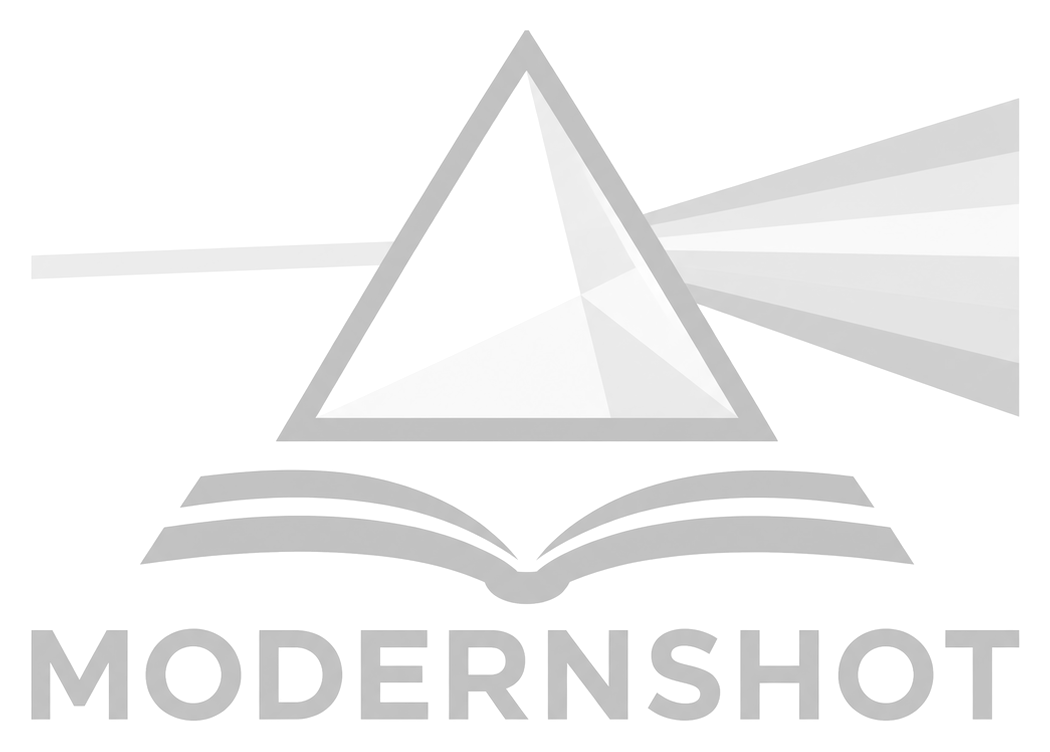
\includegraphics[width=0.55\textwidth]{logo.png}\par
\vfill
{\large 2026 年第一学期期中（开卷）\par}
\vspace{0.3cm}
{\small 课件页码标注：[F1-p$n$] 傅里叶光学 I；[F2-p$n$] 傅里叶光学 II；[F3-p$n$] 傅里叶光学 III；[VO-p$n$] 视光学（PDF 文件页码）\par}
\vspace{2cm}
\end{titlepage}

\chapter*{使用说明}
\addcontentsline{toc}{chapter}{使用说明}
\begin{idea}[零基础怎么用这本书（没学过物理光学、几何光学也忘了，从这里开始）]
\begin{enumerate}
\item \textbf{先读第零章}「零基础入门」（第 \pageref{ch:primer} 页，约 1 小时）：用信号与系统的语言讲清每个概念是什么、为什么，每节一张图。读完就能看懂题干在说什么。
\item \textbf{再看第 9 章每道往年题前的「读题」框}（\icoI\,【直觉】框）（从第 \pageref{rd:2024-1} 页起）：题干逐句翻译成大白话，生词附入门页和详解页，说明这道题是信号与系统里的什么问题、每一问要交什么。
\item \textbf{然后按下面的「题型索引」查详细推导}：每类题都有公式框、套路和可以照抄的答卷。
\item \textbf{考场上}：先用第 \pageref{fig:dectree} 页的「解题决策树」或书末「题干信号词表」（第 \pageref{tab:signal} 页）判断题型；遇到不认识的词查术语表（第 \pageref{tab:glossary} 页，按拼音排序，一句话白话 + 信号与系统对应物 + 关键公式 + 页码）。
\end{enumerate}
\end{idea}
\begin{itemize}
\item \textbf{五种框}：靠\textbf{标题前的图标、标题里的文字标签、边框样式}区分（黑白打印也分得清），见下面的图例。
\item \textbf{查找顺序}：① 本页「题型索引」$\to$ ② 章节目录 $\to$ ③ 文末「公式框一览」$\to$ ④ 文末关键词索引（按拼音排序）。
\item \textbf{记号}：傅里叶变换核 $\exp[-i2\pi(ux+vy)]$；$\sinc(x)=\sin(\pi x)/(\pi x)$；透镜相位 $\exp\!\left(-ik\frac{x^2+y^2}{2f}\right)$；输入面 $(x_1,y_1)$，输出面 $(x,y)$。与课件一致。
\end{itemize}


\subsection*{五种框的图例}
{\small
\begin{tcbraster}[raster columns=2,raster equal height=rows,raster column skip=4mm,raster row skip=3mm]
\begin{tcolorbox}[fmlstyle,unbreakable,title={\icoF\ 【公式 F$n$】标题}]
\textbf{公式框}：黑底白字标题 + 粗实线框，图标 \ding{110}（实心方块）。\\
里面是\textbf{可以直接抄的公式和结论}，全书连续编号，书末有「公式框一览」。\\
\textsf{什么时候看}：考场上要用某个公式时。
\end{tcolorbox}
\begin{tcolorbox}[rcpstyle,unbreakable,title={\icoR\ 【套路 $n$】标题}]
\textbf{套路框}：左边一条粗黑边，图标 \ding{228}（箭头）。\\
里面是\textbf{解题步骤}，按 ①②③ 照着写就是答卷，书末有一览。\\
\textsf{什么时候看}：认出题型以后，照它一步步做。
\end{tcolorbox}
\begin{tcolorbox}[warnstyle,unbreakable,title={\icoW\ 【易错】标题}]
\textbf{易错框}：双线框 + 浅灰底，图标是带感叹号的三角。\\
里面是\textbf{最容易抄错的符号、系数、约定}。\\
\textsf{什么时候看}：答案写完，交卷前对照检查。
\end{tcolorbox}
\begin{tcolorbox}[ideastyle,unbreakable,title={\icoI\ 【直觉】标题}]
\textbf{直觉框}：虚线框、标题没有底色，图标是灯泡。\\
里面是\textbf{大白话讲为什么}；第 9 章每道题前的「读题」也是这种框。\\
\textsf{什么时候看}：复习时看；考场上可以跳过（「读题」除外）。
\end{tcolorbox}
\begin{tcolorbox}[examstyle,unbreakable,title={\icoE\ 【例】标题}]
\textbf{例题框}：灰底标题 + 细线框，图标 \ding{46}（铅笔）。\\
里面是\textbf{例题、往年题的完整答卷}，可以照抄格式。\\
\textsf{什么时候看}：做同类题时对照着写。
\end{tcolorbox}
\begin{tcolorbox}[enhanced,colback=white,frame hidden,unbreakable,left=2pt]
\textbf{图里的线}：全书的图不靠颜色区分，靠\textbf{线型}（实线、虚线、点线、点划线）、粗细和旁边的文字标注；图注里说的「实线」「虚线」就是指这些。
\end{tcolorbox}
\end{tcbraster}}

\clearpage
\section*{解题决策树}\phantomsection\label{fig:dectree}
\addcontentsline{toc}{section}{解题决策树}
\noindent 拿到题目，先圈出题干里的关键词，从上往下走：\textbf{第 1 步}判断这道题在算什么（左列），\textbf{第 2 步}在右列找到具体情况，翻到页码处的套路照做。关键词对照更全的表在第 \pageref{tab:signal} 页。

\begin{center}
\begin{tikzpicture}[>=Stealth,font=\small,
  cat/.style={draw=#1!60!black,fill=#1!10,rounded corners=3pt,text width=4.0cm,align=left,inner sep=4pt,line width=0.6pt},
  det/.style={draw=gray!55,fill=white,rounded corners=3pt,text width=10.5cm,align=left,inner sep=4pt},
  pg/.style={color=blue!50!black}]
\node[draw=blue!50!black,fill=blue!6,rounded corners=3pt,text width=15.6cm,align=center,inner sep=5pt,line width=0.7pt] (root) at (0,0)
 {\sffamily\bfseries 第 1 步：这道题在算什么？\quad\normalfont\small（相干 / 非相干先判断清楚：激光、单色相干 $\to$ 算复振幅；普通光、荧光、MTF $\to$ 算强度）};

\node[det,anchor=north east] (d1) at ([yshift=-7mm]root.south east)
 {$\bullet$ 写透射系数 $t=\exp[ik(n-1)\Delta]$：p.\,\pageref{sec:screens}\quad
  $\bullet$ 凑成 $-\frac{k r^2}{2F}$ 读焦距：p.\,\pageref{sec:equivlens}\\
  $\bullet$ 三次面型平移（Alvarez）：p.\,\pageref{sec:alvarezi}\quad
  $\bullet$ 两束光干涉条纹：p.\,\pageref{sec:twobeam}};
\node[cat=orange,anchor=east] (c1) at ([xshift=-5mm]d1.west)
 {\textbf{① 元件相位 / 等效透镜}\\\scriptsize 面型、厚度、折射率、复透过率、“等效于透镜”};

\node[det,anchor=north] (d2) at ([yshift=-4mm]d1.south)
 {$\bullet$ 傍轴 / 远场哪个难、菲涅耳 / 夫琅禾费用了什么近似：p.\,\pageref{box:approx}\\
  $\bullet$ 推导衍射公式：p.\,\pageref{sec:diffderiv}\quad
  $\bullet$ 孔径远场图样六步：p.\,\pageref{sec:fraunrecipe}\\
  $\bullet$ 传播 $z$ 后的场（角谱）、Talbot：p.\,\pageref{sec:angspec}};
\node[cat=teal,anchor=east] (c2) at ([xshift=-5mm]d2.west)
 {\textbf{② 传播 / 衍射}\\\scriptsize 距离 $z$、球面波、傍轴、远场、菲涅耳、夫琅禾费};

\node[det,anchor=north] (d3) at ([yshift=-4mm]d2.south)
 {$\bullet$ 单透镜焦面场、谱点位置：p.\,\pageref{sec:focalplane}\quad
  $\bullet$ 4f 输出、放大率、级联：p.\,\pageref{sec:4fderiv}\\
  $\bullet$ 频谱面放滤波器求 CTF：p.\,\pageref{sec:4fctf}\quad
  $\bullet$ 光栅挡级：p.\,\pageref{sec:gratingfilter}\\
  $\bullet$ 频谱面线性相位 / SLM：p.\,\pageref{sec:linphase}\quad
  $\bullet$ 物偏离焦面 $x_2=M^2x_1$：p.\,\pageref{sec:4foffset}\\
  $\bullet$ 相衬、暗场：p.\,\pageref{sec:phasecontrast}\quad
  $\bullet$ 显微镜、倾斜照明：p.\,\pageref{sec:abbe}};
\node[cat=green,anchor=east] (c3) at ([xshift=-5mm]d3.west)
 {\textbf{透镜与 4f}\\\scriptsize 前 / 后焦面、频谱面、4f、滤波器、SLM、级联};

\node[det,anchor=north] (d4) at ([yshift=-4mm]d3.south)
 {\textbf{相干？}$\to$ CTF = 光瞳，截止 $\frac{\mathrm{NA}}{\lambda}$：p.\,\pageref{sec:typeA}\\
  \textbf{非相干？}$\to$ OTF = 光瞳自相关，截止 $\frac{2\mathrm{NA}}{\lambda}$：方瞳 / 圆瞳 p.\,\pageref{sec:typeB}；几条缝 / 几个孔 p.\,\pageref{sec:typeC}\\
  $\bullet$ 求 PSF：p.\,\pageref{sec:typeD}\quad
  $\bullet$ 条纹对比度 $K$：p.\,\pageref{sec:typeE}\quad
  $\bullet$ 离焦：p.\,\pageref{sec:typeG}\\
  $\bullet$ 采样、混叠：p.\,\pageref{sec:typeF}\quad
  $\bullet$ SIM 超分辨：p.\,\pageref{sec:sim}};
\node[cat=blue,anchor=east] (c4) at ([xshift=-5mm]d4.west)
 {\textbf{③ 成像：PSF / MTF}\\\scriptsize 出射光瞳、衍射受限、截止频率、MTF、对比度};

\node[det,anchor=north] (d5) at ([yshift=-4mm]d4.south)
 {$\bullet$ 证 $S\approx1-k^2\sigma_W^2$、$\lambda/14\Rightarrow0.8$：p.\,\pageref{ex:strehl-tplA}\quad
  $\bullet$ 证 $S\approx\ee^{-k^2\sigma_W^2}$：p.\,\pageref{ex:strehl-tplB}\\
  $\bullet$ 证有像差 MTF 不升、何种 $W$ 不降：p.\,\pageref{sec:mtfproof}\\
  $\bullet$ 给 $W(\rho,\theta)$ 求 RMS：p.\,\pageref{rc:rms}\quad
  $\bullet$ 最佳补偿：p.\,\pageref{rc:balance}\quad
  $\bullet$ 离焦换算：p.\,\pageref{sec:defocus-units}};
\node[cat=red,anchor=east] (c5) at ([xshift=-5mm]d5.west)
 {\textbf{④ 像差 / Strehl}\\\scriptsize 波像差 $W$、RMS、$\sigma_W$、Strehl、$\lambda/14$};

\node[det,anchor=north] (d6) at ([yshift=-4mm]d5.south)
 {$\bullet$ 透镜成像位置、大小：p.\,\pageref{sec:lensimg}\quad
  $\bullet$ 远点近点、配镜：p.\,\pageref{sec:farpoint}, \pageref{sec:correct}\\
  $\bullet$ 光阑与光瞳作图：p.\,\pageref{sec:stops}\quad
  $\bullet$ CPD、视网膜屏：p.\,\pageref{sec:screencpd}\quad
  $\bullet$ 视力：p.\,\pageref{sec:acuity}\\
  $\bullet$ gamma 灰阶：p.\,\pageref{sec:gammacalc}\quad
  $\bullet$ 光度单位、朗伯、正弦条件：p.\,\pageref{sec:photounits}, \pageref{sec:abbesine}};
\node[cat=violet,anchor=east] (c6) at ([xshift=-5mm]d6.west)
 {\textbf{视光学 / 光度}\\\scriptsize 眼、屈光度、远点、视力、CPD、gamma、亮度、朗伯};

\foreach \i in {1,...,6} \draw[->,thick,gray!70] (c\i.east)--(d\i.west);
\coordinate (trunk) at ([xshift=-4mm]c1.west);
\draw[thick,blue!50!black] (root.south -| trunk) -- (c6.west -| trunk);
\foreach \i in {1,...,6} \draw[->,thick,blue!50!black] (c\i.west -| trunk) -- (c\i.west);

\node[draw=blue!50!black,fill=blue!6,rounded corners=3pt,text width=15.6cm,align=left,inner sep=5pt,anchor=north east] (fin) at ([yshift=-7mm]d6.south east)
 {\sffamily\bfseries 第 2 步\normalfont\small：在页码处照【套路】框一步步写。\quad
  \sffamily\bfseries 第 3 步\normalfont\small：翻第 9 章同类往年答卷（第 \pageref{ch:exams} 页起）对照格式。\\
  \sffamily\bfseries 卡住了\normalfont\small：题干的词看不懂 $\to$ 术语表 p.\,\pageref{tab:glossary}；概念想不通 $\to$ 第零章 p.\,\pageref{ch:primer}；不知道是哪类题 $\to$ 信号词表 p.\,\pageref{tab:signal}。};
\end{tikzpicture}
\end{center}
\clearpage

\section*{题型索引}\label{tab:typeindex}
\par\renewcommand{\arraystretch}{1.35}
\begin{longtable}{@{}P{6.4cm}P{6.2cm}r@{}}
\toprule
题目长什么样 & 去看 & 页码\\ \midrule
\endhead
\textbf{看不懂题目里的概念} & 第零章（零基础入门）、术语表 & \pageref{ch:primer}, \pageref{ch:glossary}\\
\textbf{不知道是哪类题} & 解题决策树、题干信号词表 & \pageref{fig:dectree}, \pageref{tab:signal}\\
\multicolumn{3}{@{}l}{\rule{0pt}{14pt}\sffamily\bfseries\color{blue!50!black}【傅里叶变换与基础】}\\
求某个图形 / 孔的傅里叶变换 & 变换对表、性质表、可抄证明 & \pageref{sec:pairs}, \pageref{sec:ftproofs}\\
单缝、多缝、阵列、余弦 / 黑白光栅的频谱 & 题型例题（缺级、各级强度）& \pageref{sec:ftexamples}\\
卷积、相关怎么算怎么画 & 分段推导、多缝自相关 & \pageref{sec:convcalc}\\
平面波方向 $\leftrightarrow$ 空间频率 & 空间频率 & \pageref{sec:spfreq}\\
两束光干涉的条纹频率、对比度 & 两束平面波干涉 & \pageref{sec:twobeam}\\
写出光屏的复透射系数 & 九种光屏速查 & \pageref{sec:screens}\\
采样定理、sinc 插值、DFT 尺度 & 数学工具 & \pageref{sec:sampling}\\
\multicolumn{3}{@{}l}{\rule{0pt}{14pt}\sffamily\bfseries\color{blue!50!black}【衍射】}\\
判断傍轴 / 远场 / 菲涅耳 / 夫琅禾费（2025-1）& 定量比较、答题模板 & \pageref{box:approx}, \pageref{ex:2025-1-diff}\\
推导菲涅耳 / 夫琅禾费公式 & 逐步推导 & \pageref{sec:diffderiv}\\
自由传播后的场（角谱）、Talbot 自成像 & 角谱传递函数、例题 & \pageref{sec:angspec}, \pageref{ex:talbot}\\
孔径的远场图样、艾里斑、双缝缺级 & 解题六步、例题 & \pageref{sec:fraunrecipe}, \pageref{ex:slit}\\
\multicolumn{3}{@{}l}{\rule{0pt}{14pt}\sffamily\bfseries\color{blue!50!black}【透镜与 4f】}\\
某个相位分布等效于什么透镜 & 等效透镜 & \pageref{sec:equivlens}\\
为什么后焦面是傅里叶变换（推导）& 6 步推导 & \pageref{sec:lensFTderiv}\\
物在透镜前 $d_0$ / 后方，焦面场、谱点位置 & 焦面复振幅 & \pageref{sec:lensFT}, \pageref{sec:focalplane}\\
4f 输出、放大率、级联（2024-4）& 4f 推导、模板 & \pageref{sec:4fderiv}, \pageref{ex:2024-4}\\
频谱面滤波器 $\to$ 相干传递函数 & 滤波求 CTF & \pageref{sec:4fctf}\\
输入光栅、挡掉某几级求输出 & 光栅滤波 & \pageref{sec:gratingfilter}\\
频谱面加线性相位 / 输出平移 & 线性相位 & \pageref{sec:linphase}\\
4f 物偏离焦面 $x_2=M^2x_1$（2024-5）& 偏离补偿、完整证明 & \pageref{sec:4foffset}, \pageref{ex:2024-5}\\
Alvarez / Lohmann 变焦透镜（2025-3）& 平移版、4f 版 & \pageref{sec:alvarezi}, \pageref{sec:alvarezii}\\
光学加减法、相衬、暗场 & 相干光学处理 & \pageref{sec:addsub}, \pageref{sec:phasecontrast}\\
\multicolumn{3}{@{}l}{\rule{0pt}{14pt}\sffamily\bfseries\color{blue!50!black}【成像（PSF / CTF / OTF / MTF）】}\\
相干截止频率（像方 / 物方）& 题型 A & \pageref{sec:typeA}\\
方瞳、圆瞳的 OTF 与画图 & 题型 B & \pageref{sec:typeB}\\
分块光瞳（多缝）画 MTF（2025-2）& 题型 C、三缝例 & \pageref{sec:typeC}, \pageref{ex:3slit}\\
由光瞳求 PSF & 题型 D & \pageref{sec:typeD}\\
条纹对比度传递 & 题型 E & \pageref{sec:typeE}\\
像元采样、双折射低通滤波器 & 题型 F & \pageref{sec:typeF}\\
离焦 OTF、对比度反转、弥散圆 & 题型 G & \pageref{sec:typeG}\\
证明像差使 MTF 下降 / 等号条件（2024-1）& 施瓦茨不等式 & \pageref{sec:mtfproof}, \pageref{ex:2024-1}\\
SIM、频谱搬移、超分辨（2024-3）& SIM 全流程 & \pageref{sec:sim}, \pageref{ex:2024-3}\\
阿贝成像、显微镜分辨率、倾斜照明 & 阿贝成像 & \pageref{sec:abbe}\\
\multicolumn{3}{@{}l}{\rule{0pt}{14pt}\sffamily\bfseries\color{blue!50!black}【像差与 Strehl】}\\
证明 $S\approx1-k^2\sigma_W^2$（2024-2）& 答题模板 A & \pageref{ex:strehl-tplA}, \pageref{ex:2024-2}\\
证明 $S\approx\exp(-k^2\sigma_W^2)$（2025-4）& 答题模板 B & \pageref{ex:strehl-tplB}, \pageref{ex:2025-4}\\
Strehl 数值计算、反查、变式 & 数值表、变式套路 & \pageref{sec:strehl-num}, \pageref{rc:strehl-variants}\\
给 $W(\rho,\theta)$ 求 RMS、最佳补偿 & 求 RMS、线性回归 & \pageref{sec:aberrms}, \pageref{rc:balance}\\
离焦量换算、焦深 & 四种表示 & \pageref{sec:defocus-units}\\
Zernike 系数、人眼像差 & Zernike & \pageref{sec:zernike}\\
波像差与光线像差、Shack-Hartmann & 光线像差 & \pageref{sec:rayaberr}\\
\multicolumn{3}{@{}l}{\rule{0pt}{14pt}\sffamily\bfseries\color{blue!50!black}【视光学】}\\
单透镜成像、放大率 & 成像与透镜 & \pageref{sec:lensimg}\\
透镜组、基点作图、逐次成像 & 透镜组 & \pageref{sec:lenscombo}\\
视网膜像大小、调节量 & 视网膜像 & \pageref{sec:retimg}\\
由眼轴求远点 / 近点 & 屈光不正 & \pageref{sec:farpoint}\\
配镜度数、框架 $\leftrightarrow$ 隐形换算 & 配镜推导 & \pageref{sec:correct}\\
老花、看清范围、读处方 & 老花、处方 & \pageref{sec:presby}, \pageref{sec:rx}\\
放大镜、望远镜、出瞳与适眼距 & 目视仪器 & \pageref{sec:magnifier}, \pageref{sec:telescope}\\
孔径光阑、入瞳出瞳、视场光阑、作图 & 光阑与光瞳 & \pageref{sec:stops}, \pageref{sec:stopswitch}\\
屏幕 PPD / CPD、视网膜屏、所需 ppi & 空间分辨 & \pageref{sec:screencpd}\\
视力表换算 & 视力 & \pageref{sec:acuity}\\
眼的衍射截止、视锥采样 & 眼的衍射极限 & \pageref{sec:eyediff}\\
CSF 与 MTF 联立作图 & 联立套路 & \pageref{sec:mtfcsf}\\
gamma、sRGB 灰阶 $\leftrightarrow$ 亮度 & 灰阶计算 & \pageref{sec:gammacalc}\\
零阶保持频谱、混叠、量化、运动模糊 & 显示器 & \pageref{sec:zoh}, \pageref{sec:alias}\\
\multicolumn{3}{@{}l}{\rule{0pt}{14pt}\sffamily\bfseries\color{blue!50!black}【光度与色度】}\\
光度学单位换算 & 单位关系 & \pageref{sec:photounits}\\
朗伯体光通量（小测计算 1）& 逐步积分 & \pageref{sec:lambert}\\
阿贝正弦条件、亮度守恒（小测计算 2）& 傅里叶证法 & \pageref{sec:abbesine}, \pageref{sec:luminance}\\
色度坐标计算 & 色度 & \pageref{sec:color}\\
\multicolumn{3}{@{}l}{\rule{0pt}{14pt}\sffamily\bfseries\color{blue!50!black}【往年原题】}\\
2024 期中 / 2025 随堂 / 2024 小测 & 完整答卷 & \pageref{sec:ex2024}, \pageref{sec:ex2025}, \pageref{sec:quiz2024}\\
\bottomrule
\end{longtable}

\tableofcontents
